q%!TEX root = sib_prog_eval_two_columns.tex

\section*{Introduction}

In the past decade, the study of ecology and evolution has been greatly facilitated by the use of genetic 
data.  Many early uses of genetic data focused on genetic variation at the level of populations, 
studying allele frequencies from different locations \citep{neigel97}. With today's abundant and 
inexpensive genetic resources, however, genetic data are increasingly applied to study ecology at the 
level of individuals within populations \citep{Pea&Cra2004,Maneletal2005}. One important example is the 
inference of pedigree relationships between individuals sampled from the wild 
\citep{blouin03,Pemberton2008}. Pedigree inference approaches have been used to study a wide range of 
phenomena from multiple paternity \citep{Sogardetal2005} and aggregation of closely related kin 
\citep{Fraseretal2005}  to inbreeding \citep{Marshalletal2002} and fitness-associated quantitative 
trait loci \citep{beraldi07}. 

Relationship inference can take place at an intergenerational scale, with problems ranging from 
establishing multiple paternity in a few clutches of turtles \citep{Pea&Avi2001} all the way up to 
reconstructing multigenerational pedigrees of nearly all the members of intensively studied populations 
\citep{Robinsonetal2006,Dunnetal2011}.  And, relationship inference can take place at the intragenerational scale when the relationship between members of a single generation must be inferred, 
without knowledge of their parents or ancestors.  Initially, the problem of intragenerational inference 
was treated in terms of the relationships between pairs of individuals \citep{Thompson1975}; 
however, this is not the most powerful way to approach the problem, and today several methods have been 
proposed that make joint inference of the intragenerational relationships between more than two members 
of a sample \citep{painter97,almudevar99,Siebertsetal02,Wang2007_triadic}.  

When a single cohort of individuals can be reliably sampled together as a group, a special case of 
joint (as opposed to pairwise) relationship inference known as ``sibship inference'' is possible.  In 
sibship inference it is assumed that all the members of a sample are of a single generation and are 
related as either full or half siblings, or are otherwise unrelated. This type of scenario occurs 
frequently in molecular ecology, especially in the study of fecund organisms such as fish 
\citep{And&Dun2008,Garzaetal_norcal}, amphibians \citep{Halversonetal2006}, or invertebrates \citep{read12} that are 
easily sampled during an early life stage that can be distinguished from reproductively-mature life 
stages.  The goal of sibship inference is typically a partition of the sample into groups that are full 
siblings. Some of the methods available today also aim to infer half sibling clusters.  

Starting with \citet{painter97} there have been a number of methods proposed for sibship inference.  
Some of these methods are based entirely on the likelihood of a partition 
\citep{painter97,thomas02,wang04,wang09}; others rely on multiallelic markers, Mendelian compatibility, 
and heuristic optimality criteria \citep{konovalov04,bergerwolf07,sheik08}; one  uses graph-theoretic 
approaches to find a partition from pairwise likelihood information \citep{beyer03}; two use 
approximations to the full likelihood of a partition \citep{Smithetal2001,Wang2012pairwise}; and one 
uses considerations of Mendelian compatibility paired with likelihood-based criteria 
\citep{almudevar99}. 

\citet{butler04} assessed the accuracy of four different methods of sibship reconstruction on simulated 
and real data sets with varying true arrangements of full siblings and numbers of markers and alleles. 
Since their paper, several new methods have been developed and presented in the literature.  The 
authors of these new methods typically evaluate their performance with a simulation study.  
Unfortunately, these simulations do not always provide informative comparisons of the relative 
performance of different methods. In some cases, only the newly-developed method is evaluated, and no 
other competing methods are included in the simulations \citep{beyer03,wang04,wang09}.  In other cases, 
several competing methods are evaluated, but the simulations may not include the best methods for 
comparison \citep{bergerwolf07}, they may be too limited in scope (in terms of number of alleles, loci, 
or true relationship configurations) to provide suitable distinction between the methods 
\citep{alm&and11,ashley09}, or they use a performance criterion that unfairly favors their own new 
method (\citealt{bergerwolf07,chaovalitwongse07,ashley09}, see below).  As a consequence, molecular 
ecologists may currently feel confused by their choices for sibship inference software and have little 
idea about which packages are likely to perform well in their particular research systems. 

In this paper, we assess the performance of several prominent sibship inference methods across a broad 
range of conditions.  Our goals are threefold. First, we hope to allow end users of the software to 
discern which methods will be most suitable for their own projects and to predict the accuracy they 
might expect.  Second, looking at the relative performance of methods across a broad range of 
conditions brings us a better understanding of the tradeoffs of different methods, which suggests ways 
that methods may be improved in the future. And finally, having summarized a considerable amount of 
program output, we provide guidance on the interpretation of results from sibship inference.
  

\section*{Methods}
\subsection*{Simulated Data}
We simulated samples of genetic data from 10 different scenarios that varied in the number and 
arrangement of full and half siblings.  The first nine of these scenarios, which we collectively refer 
to as the $n75$ scenarios, involved samples of $n=75$ individuals, including three (\nosibs{}, 
\allhalf{}, \allpathalf) that have no full siblings, but vary in the number and arrangement of half 
siblings; two that include many small full sibling groups (\sfsnoh{}, \sfswh{}); two that are dominated 
by several large full sibling groups (\slfsgnoh{}, \slfsgwh{}); and two that include one large full 
sibling group (\onelargenoh{}, \onelargewh{}).  Of the latter six configurations, half of them include 
no half-siblings, and the remainder (denoted by a trailing ``\_H'' in their names) include half 
siblings.   The relationship of the sampled individuals in each of these nine scenarios appears in 
\FIG~\ref{fig:confs}.

%\begin{equation}
%\mbox{FIGURE ped\_configs\_figure.pdf}\label{fig:confs}
%\end{equation}
\begin{figure*}
\begin{center}
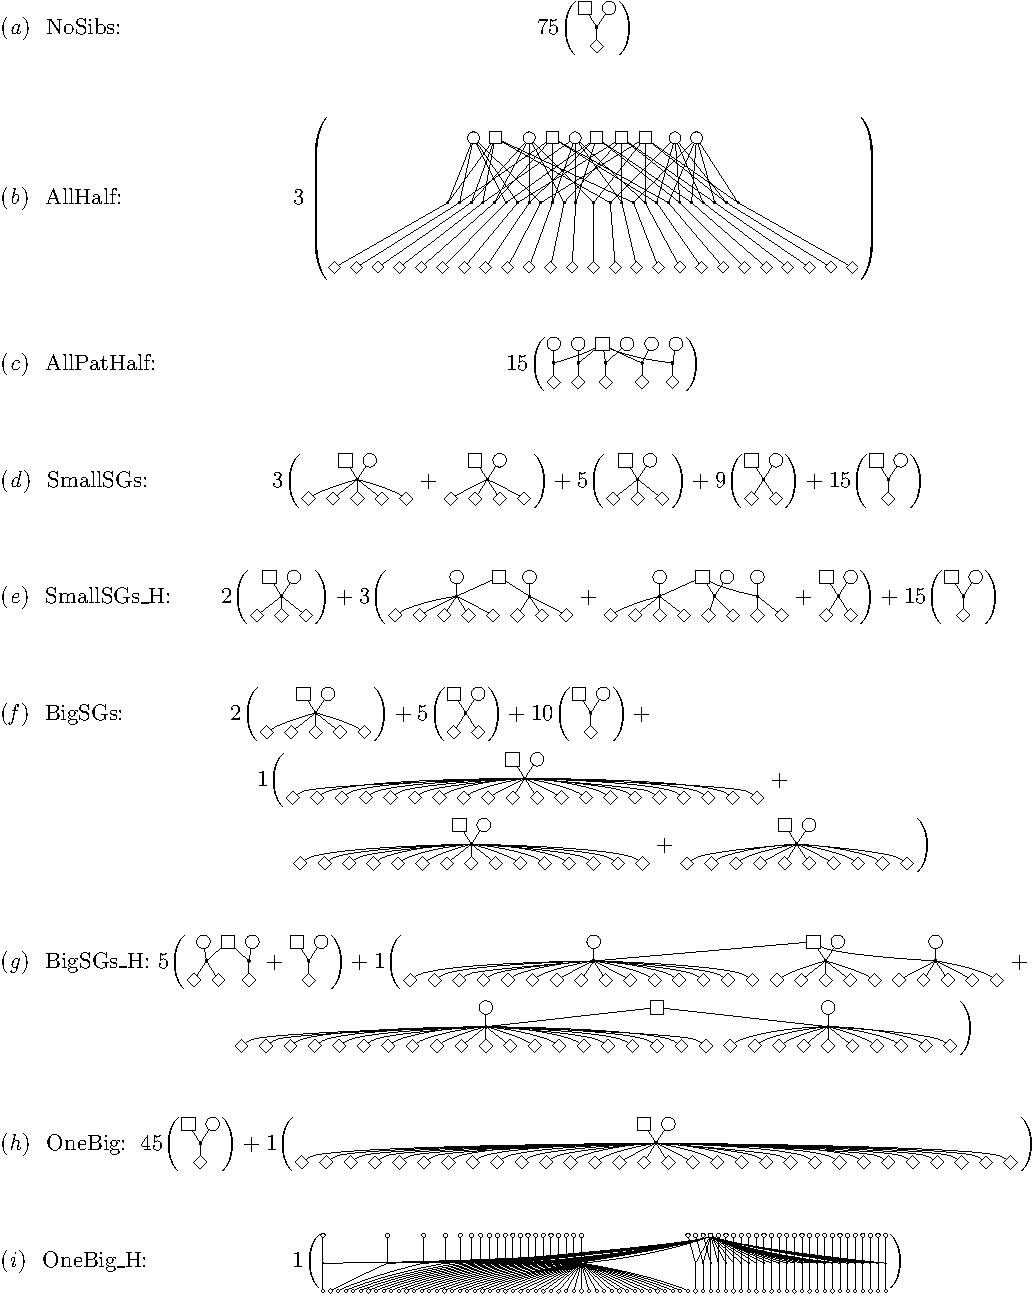
\includegraphics[width=.90\textwidth]{images/ped_configs_figure.pdf}
\end{center}
\newcommand{\confscaption}{Configuration of relationships in simulated samples of 75 individuals.  Individuals in samples 
are represented by diamonds.  They are connected to their mothers and fathers (circles and boxes, 
respectively) by a marriage-node representation of the pedigree \protect\citep{Lau&She2003}. Founders in the 
pedigree are all unrelated.}
\caption[\confscaption]{\sometimes{\confscaption}}
\label{fig:confs}
\end{figure*}
The tenth scenario (\lottalarge) involved a sample of 390 individuals belonging to a number of large 
full sibling groups with no half siblings.  In particular, there was a single full sibling group of 
each of the following sizes: 150, 100, 70, 40, 20, 10.

We used the C program {\sc nookie} (written by ECA and available at \url{https://github.com/eriqande/nookie}) to simulate each of the data sets.  
{\sc nookie} is given a set of allele frequencies at a number of loci and first simulates individual 
genotypes (with no Hardy-Weinberg or linkage disequilibrium) into a parental generation.  It then mates 
those parents together and produces offspring via Mendelian segregation in a manner that can be fully 
specified by the user.  For each simulated data set, the allele frequencies at every locus were given 
by the Zipf distribution (at a locus with $A$ alleles, the frequency of allele $a$ is proportional to 
$1/a$ for $a=1,\ldots,A$). We simulated data using 5 different values $(5,10,15,20,25)$ for the number 
of alleles, $A$, at each locus. For each combination of the 5 values of $A$ and the 10 relationship 
configurations we simulated 50 data sets (2,500 in total)  with 25 unlinked loci and no genotyping 
error.  

From each of these 2,500 data sets, two additional data sets were created, one with genotyping error 
rate parameters $d=0.02$,~$m=.01$ and the other with $d=0.07$,~$m=0.03$.  Parameter $d$ is the rate of dropout 
errors and $m$ of miscall errors.  At each locus in each individual, independently, with probability $d
+m$ a genotyping error was simulated. With probability $\frac{d}{d+m}$ a randomly chosen gene copy at 
the locus was censored so that the genotype appeared as a homozygote of the allelic type of the 
remaining gene copy; with probability $\frac{m}{d+m}$ a randomly selected gene copy at the locus was 
changed to a different allelic type.  If the type of the original allele was represented by $\ell_
\mathrm{true}$, then the type after miscall, $\ell_\mathrm{err}$, was found by simulating random 
variables $\delta$ (1 or -1 with equal probability) and $S$ (Poisson random variable with mean 1) until 
$\ell_\mathrm{err} = \ell_\mathrm{true}+\delta(1+S)$ and $\ell_\mathrm{err}>0$. (In other words, 
miscall errors were more likely to be made to alleles of similar type, approximating the miscoring of 
microsatellite allele lengths).  

Once these 7,500 data sets with 25 loci had been simulated, we used them to create data sets with 5 
different values $(5,10,15,20,25)$ of the number of loci, $L$, by including just the first $L$ of the 
25 loci in the data set.  Hence, we had 37,500 different data sets on which to compare the accuracy of 
sibship inference programs.  The different simulation conditions are summarized in Table~
\ref{tab:parsum}
\begin{table*}
\begin{center}
\caption{Simulation conditions.  10 relationship configurations were simulated. For each one, data sets 
were simulated with all possible combinations of the number of alleles, number of loci, and genotyping 
error rates. \label{tab:parsum}}
\resizebox{\textwidth}{!}{%
\begin{tabular}{lccl}
\hline
Relationship Configuration (10) & ~~No.~of Alleles (5)~~ & ~~No. of Loci (5)~~ & Genotyping Error (3)\\ 
\hline
\nosibs, \allhalf, \allpathalf,          &     5    &     5     &    None $(d=0,\ m=0)$     \\
\sfsnoh, \sfswh,        &    10    &     10    &    Low  $(d=0.03,m=0.01)$     \\
\slfsgnoh, \slfsgwh,       &    15    &     15    &    High $(d=0.07,m=0.03)$     \\
\onelargenoh, \onelargewh,         &    20    &     20    &         \\
\lottalarge          &    25    &     25   &         \\
\hline
\end{tabular}
}
\end{center}
\end{table*}




\subsection*{Inference Programs}
We analyzed the simulated data using four different programs: \colony{} \citep{wang04,wang09, 
Wang2012pairwise}, \prt~V2.2 \citep{almudevar99,alm&and11}, \kinalyzer{} 
\citep{bergerwolf07,ashley09,sheik08}, and \familyfinder{} \citep{beyer03}.  These methods were chosen 
for their prominence in the published literature, their inclusion as sibship reconstruction methods in 
the review by \citet{jonesAG10}, and because they come with user interfaces that can be rendered 
amenable to batch processing of many data sets.  Of the remaining sibship reconstruction methods noted 
in \citet{jonesAG10} we did not assess either {\sc pedigree~2.2} \citep{Smithetal2001} or {\sc 
kingroup~2} \citep{konovalov04} because neither are suitable for application to many data sets, and we 
did not assess {\sc ml-relate} \citep{Kalinowsketal2006} because it deals exclusively with the 
estimation of pairwise relatedness.


\colony{} uses simulated annealing to search for the maximum-likelihood partition of a sample into 
collections of full siblings, possibly nested within half siblings. We initially applied \colony~{\sc 2.0} to the simulated data 
sets.  However, after we launched this simulation project, \citet{Wang2013} described significant improvements made to \colony{} 
to reduce the splitting
of large sibships \citep{alm&and11} and to better control the identification of small spurious sibling groups.  
Accordingly, we repeated the analysis using the updated
version \colony~{\sc 2.0.5.2}.  We report results for both versions of the program.  Runs of the software
\colony{} can require a considerable 
amount of time.  Therefore, in choosing program settings, we chose ones that would decrease running 
time if possible: polygamy was allowed in just a single sex, allele frequencies were not updated, run 
length was set to 1, precision was set to ``low'' but the full likelihood method was used. \colony{} 
has a well developed model for genotyping errors, allowing for both dropout errors and miscall errors. 
For most runs we set the rate of dropouts and miscalls used in \colony{}'s likelihood calculation to 
both be 0.02.  In a smaller subset of runs using \colony~{\sc 2.0} we investigated the effect of changing the genotyping error 
rate settings in \colony{} to $d=0.07,\ m=0.03$ and also to $d=0.0,\ m=0.0$.    Note that although we 
allowed \colony{} to infer half-sibling groups, we did not evaluate how well it inferred half-sibling 
groups, only how well it inferred the full sibling groups. The program \colony{} has an option to 
implement a pseudolikelihood approximation, in which the likelihood of a partition is approximated by 
the product of pairwise probabilities over individuals that occur together in the same sibship. 
\citet{Wang2012pairwise} reports that this approach is much faster than the standard \colony{} method 
and yet is more accurate than other approaches based on Mendelian incompatibility or different 
formulations of pairwise likelihood and is only slightly less accurate than the full likelihood method.  
We call this approximate \colony{} algorithm \colony{}-P and we assess its performance on a subset of 
our simulated data. 



\prt{} uses an algorithm based on Mendelian incompatibility to generate a list of maximal, feasible 
sibling groups.  These are then input to a likelihood-based procedure that infers a partition of full 
sibling groups.  For this analysis, we used a newly developed version (2.2) that allows for batch 
processing and also features an heuristic, iterative approach for handling genotyping errors. See 
Appendix~1 for information about new features in V2.2. (Note that all appendices are included in the
Supporting Information).  Settings used by
\prt{} for the analysis of the data sets here are explained in Appendix~5. 



\kinalyzer{} also uses Mendelian incompatibility to generate a list of feasible sibling groups which 
are then the input to a combinatorial optimization problem---the minimum set cover problem.  The 
solution returned by \kinalyzer{} is the fewest feasible sibling groups that ``cover'' the whole sample 
(i.e., each member of the sample is represented in at least one of the feasible sibling groups in the 
minimum set cover solution). The only option choice that must be made in running \kinalyzer{} is 
whether to use the ``2-allele'' or the ``consensus'' algorithm.  We focused on the ``2-allele'' 
algorithm because \citet{ashley09} state they, ``favour the 2-allele method implemented in 
\kinalyzer{}.''  However, we also analyzed 20\% of the simulated data sets using the consensus 
algorithm \citep{sheik08} to assess its performance and to ascertain whether it is, as the authors 
suggest, more resilient to genotyping error \citep{sheik08_err_tol}.    \kinalyzer{} runs using a web 
interface: data sets are submitted to it over the Internet, the analysis is done on a remote machine, 
and the solution is returned to the user in an email message.  We used the HTML scripting utility {\tt 
curl} (Version 7.17.1, http://curl.haxx.se) within a set of custom Unix shell scripts to automate the 
process of submitting data sets to \kinalyzer{}, and we received the results at a dedicated email 
address.     


\familyfinder{} first computes the degree of pairwise relatedness between every member of the sample, 
creates a graph in which pairs of individuals with high likelihood of being full siblings are connected 
by an edge, and then uses graph algorithms to identify likely full sibling groups as those 
subgraphs which are close to being fully connected.  We compiled this C++ program using the g++ 
compiler on Mac OS X.  The program runs on the command line and has no user-configurable options other 
than the name of the file holding the input data.    


\begin{table*}
\begin{center}
\caption{Summary of Methods and number of data sets analyzed. ``Varied Settings'' are the parameters of the inference methods that were used (not the simulation settings). ``No. Rep'' is the number of 25-locus data sets simulated for each relationship configuration, and ``Total'' is the total number of data sets analyzed over the different relationship configurations, and the diffferent values of $A$, $L$, and the degree of simulated genotyping error. \label{tab:methsum}}
\begin{tabular}{lllrr}
\hline
Software & Varied Settings~~~~~~~ & Data Scenarios & No.~Rep & Total \\ \hline
\colony~{\sc 2.0.5.2} & $d=0.02$; $m=0.02$ & $n75$ scenarios & 15 & 10,125 \\
          &                  & \lottalarge{}          & 5  &    375 \\      
\\
\colony{}-P~{\sc 2.0.5.2} & $d=0.02$; $m=0.02$ & $n75$ scenarios & 15 & 10,125 \\
            &                  & \lottalarge{}          & 5  &    375\\
 \\

\colony~{\sc 2.0} & $d=0.02$; $m=0.02$ & $n75$ scenarios & 15 & 10,125 \\
          &                  & \lottalarge{}          & 5  &    375 \\      
          & $d=0.0$; $m=0.0$ & $n75$ scenarios & 5  &    3,375 \\ 
          & $d=0.07$; $m=0.03$ & $n75$ scenarios & 5  &    3,375 \\     
 \\
\colony{}-P~{\sc 2.0} & $d=0.02$; $m=0.02$ & $n75$ scenarios & 15 & 10,125 \\
            &                  & \lottalarge{}          & 5  &    375\\
\\
\prt{}      &    See Appendix~5              & $n75$ scenarios & 15 & 10,125 \\
            &                  & \lottalarge{}          & 15  &    1,125\\
\\
\kinalyzer{}~~~ & 2-allele      &   $n75$ scenarios & 50 & 33,750 \\ 
             &               &   \lottalarge{} and $A=5$ & 50 & 750$^c$ \\ 
             & consensus      &   $n75$ scenarios  & 10 & 6,750 \\
\\
\familyfinder{}  &  none  &  all 10 scenarios  &  50  &  37,500 \\
\hline
\end{tabular}
\end{center}
{\footnotesize
$\mbox{}^a$ Datasets with $A=10$ and $L\in\{5,10\}$ \\
$\mbox{}^b$ Datasets with $A\in\{5, 10, 15, 20, 25\}$ and $L=10$ \\
$\mbox{}^c$Of these 750 data sets, only the 150 of them with 5 loci yielded results from \kinalyzer{}.  
It appears no data sets with $L>5$ were successfully completed. To avoid denying service of the 
\kinalyzer{} server to other users, we submitted no more \lottalarge{} data sets to it.   
}
\end{table*}


\subsection*{Assessment of Accuracy}
To compare the accuracy of inferred full sibling groups,  we use the Partition Distance ($\PD$) between 
the true partition of a sample into full sibling groups and the inferred partition. The PD summarizes, 
in a single number, the distance between two partitions.  If $U=\{1,\ldots,N\}$ is a collection of $N$ 
elements and $A$ and $B$ are two partitions of those elements, then $\PD(A,B)$ is defined as the 
minimum number of elements of $U$ that must be removed from both $A$ and $B$ to make $A$ and $B$ equal.  
For example, if $U=\{1,2,3,4,5\}$ represents a sample of five individuals, and $A=\{\{1\},\{2\},
\{3,4,5\}\}$ is a partition in which 3, 4, and 5 are full siblings and 1 and 2 are  
unrelated, and $B=\{\{1,2\},\{3\},\{4,5\}\}$, then $\PD(A,B) = 2$ because $A$ and $B$ can be rendered 
identical by removing two elements from each (either 1 and 3 or 2 and 3).  \citet{gusfield02} pointed 
out that the $\PD$ can be computed in polynomial time as an instance of the Assignment Problem from the 
field of combinatorial optimization, and we take that approach, using the GNU Linear Programming Kit, 
Version 4.35 (http://www.gnu.org/software/glpk/glpk.html).

In some instances, it is useful to consider the PD while ignoring sibships smaller than a certain size.  
For instance, \kinalyzer{}'s 2-allele algorithm, being based exclusively on Mendelian incompatibility, has 
no capacity to exclude any two individuals as full siblings, and consequently will infer the presence 
of many sibships of size two even when none exist.  To avoid penalizing \kinalyzer{} in this context we 
define $\PDT(A,B)$, the ``trimmed'' partition distance, to be $\PD(A',B')$ where $A'$ and $B'$ are 
obtained by removing from $A$ and $B$, respectively, all elements that occur in sets of size less than 
3 {\em in both} $A$ and $B$. As an example, if $A$ and $B$ are as given above, then $A'=\{\{3,4,5\}\}$, 
$B'=\{\{3\},\{4,5\}\}$, and $\PDT(A,B)=1$ (because $A'$ and $B'$ can be rendered identical by removing 
element 3 from both of them).  

\kinalyzer{} presents a further difficulty in computing the partition distance because it does not always 
infer a partition.  Rather, \kinalyzer{} presents its solution as a set cover, which is a collection of 
sets that include all elements of $U$, but in which some elements may appear more than once.  In other 
words, the solution that \kinalyzer{} returns may indicate that $a$ is a full sibling of $b$ and $b$ is a 
full sibling of $c$, but $c$ is not a full sibling of $a$.  This is obviously incompatible with
biology, so, to evaluate such a result, it would be natural to penalize for repeat 
occurrences of any element of $U$ in the solution.  In their series of papers, it appears 
the authors of \kinalyzer{} have never penalized their program for failing to return a partition.  To 
compare a set cover solution $C$ to the true full sibling partition, $T$, they use what we will call $
\W(C,T)$---the result of applying the Assignment Problem formulation to $T$ and $C$.     This 
formulation does not penalize set cover solutions.  So, for example, if  $U=\{1,2,3,4,5,6\}$,
$T=\{\{1,2,3\},\{4,5,6\}\}$, and $C=\{\{1,2,3,4\}, \{3,4,5,6\}\}$, then $\W(C,T)=0$, but the partition 
distance between them should be 2 (since two elements, 3 and 4, could be removed from both $T$ and $C$ 
to make them identical).    Therefore, we also evaluate set cover solutions using a quantity that 
includes a penalty for indviduals that appear in more than one sibling group in the set cover solution: 
$\PDS(T,C)= D+\PD(T^*,C^*)$ where $T^*$ and $C^*$ are what remains after the $D$ elements appearing 
more than once in $C$ are completely removed from $T$ and $C$, respectively.  We stress that if $T$ and $C$ are both 
partitions, then $\W(T,C) = \PDS(T,C)=\PD(T,C)$. 
Further discussion of this matter can be found in \citet{almudevar11}. 
We denote trimmed versions of these set-cover specific distances with $\WT$ and $\PDST$.

While the partition distance is a proper distance metric and provides a valuable scalar summary of the 
quality of a program's sibship reconstruction, it does not always reveal exactly the manner in which an 
inferred sibling  partition fails to correspond to the true partition.  For example, the PD could be 
five either because a solution incorrectly splits a single sibship of size 10 in half, or because a 
solution leaves a single individual out of each of five different true sibling groups.  For this 
reason, in Supplement~4, we include a series of plots showing the size of the largest inferred sibling 
group in each simulation as a function of the largest true sibling group in each simulation.  This 
reveals interesting patterns of the variety of ways that different programs fail to capture the true 
sibling structure and will be discussed in the results.

A recent paper introduces and advances a new metric for assessing sibship reconstructions based on 
information theoretic considerations \citep{BrownDexter2012}.  We do not use that here for reasons 
outlined in Appendix~2, which documents the new metric's shortcomings.

\section*{Results}
\subsection*{$n75$ Scenarios---Overview}
We start investigating the results by considering cases with $A=25$ and $L=15$ or $20$. These are 
data-rich situations in which we expect it should be possible to identify sibling groups very accurately.  
The boxplots of Figure~\ref{fig:boxp1} summarize the partition distance, $\PDS$, obtained by each 
method in each of the nine $n75$ scenarios. 
%%

%\begin{equation}
%\mbox{FIGURE ped\_configs\_figure.pdf}\label{fig:boxp1}
%\end{equation}

\begin{sidewaysfigure*}
\begin{center}
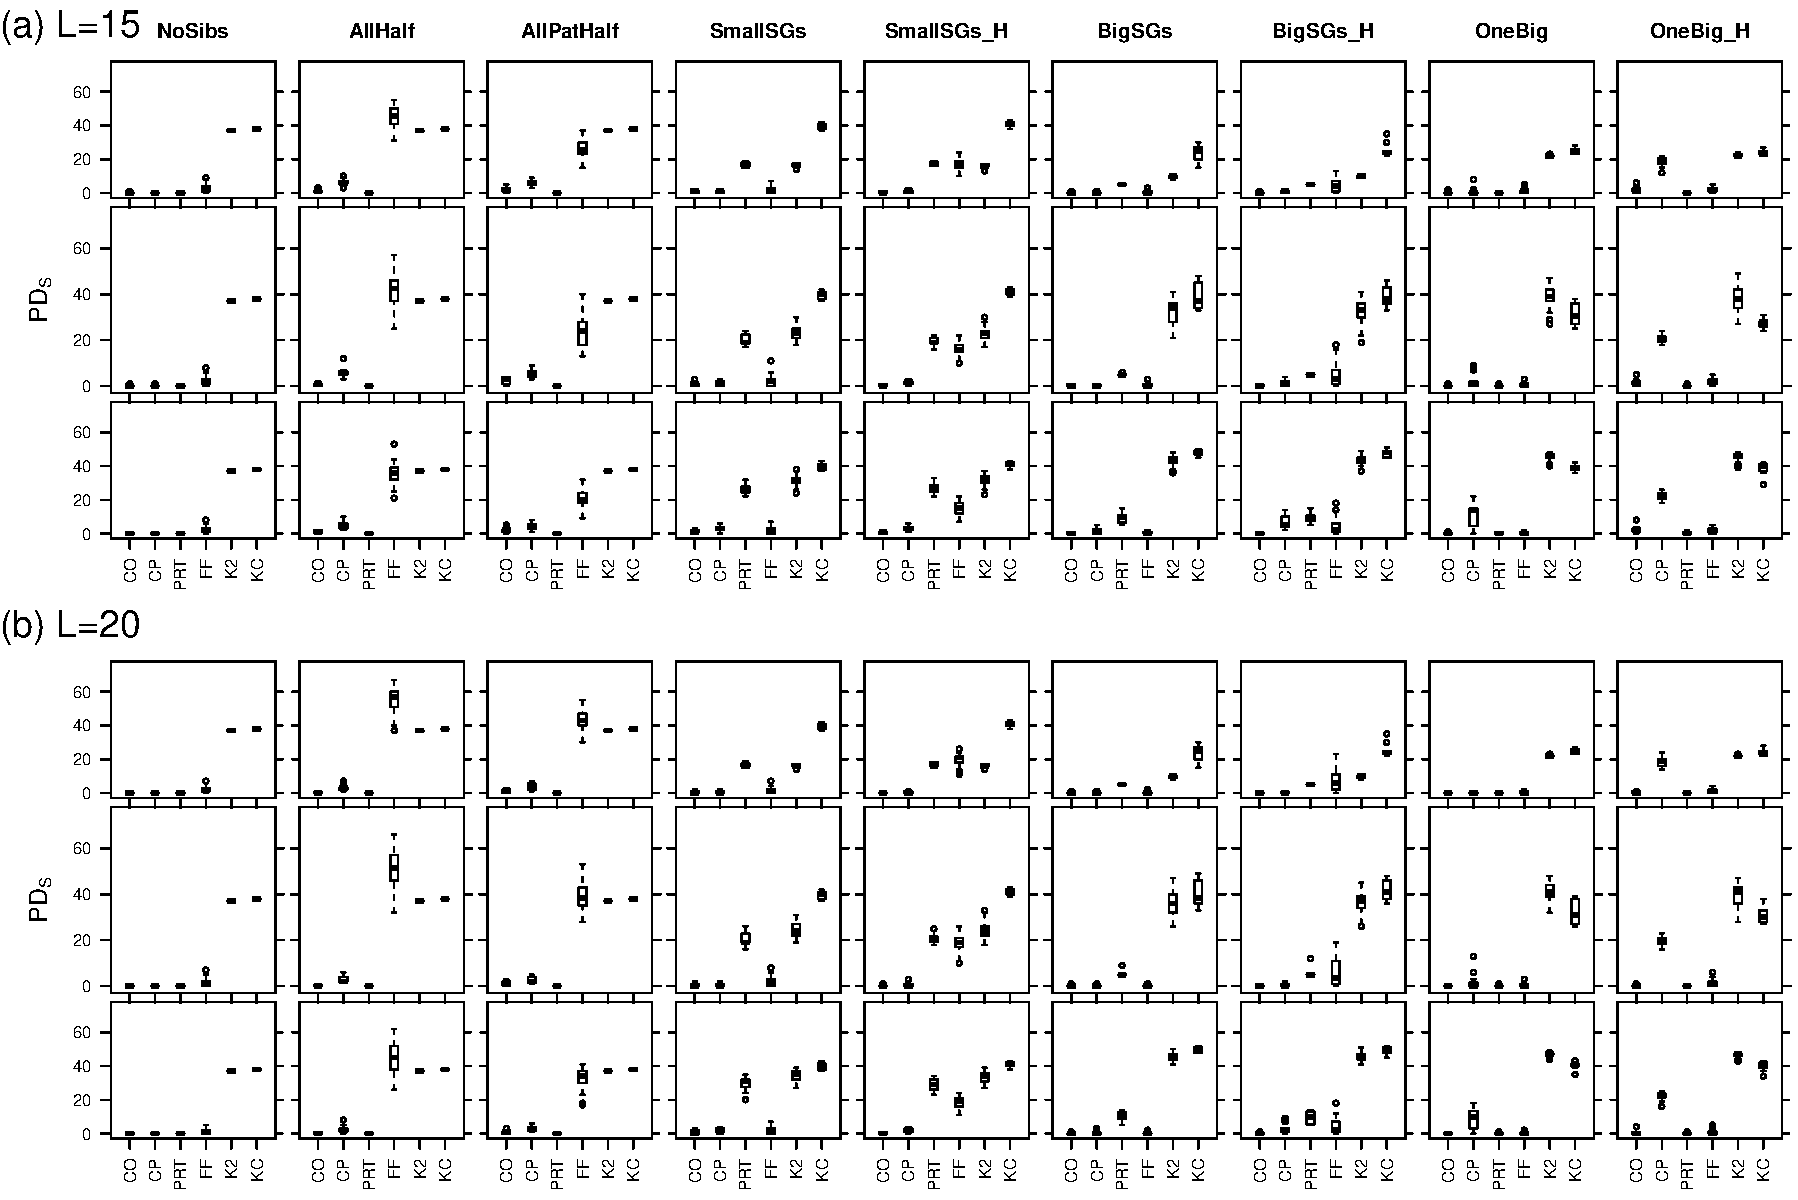
\includegraphics[width=\textwidth]{images/boxplots_for_paper25_num2.pdf}
\newcommand{\boxponecaption}{Boxplot representation of values of $\PDS$ for $A=25$ alleles and $L=15$ ({\em a}) and $L=20$ 
({\em b}) loci for all methods (CO=\colony; CP=\colony{}-P; PRT=\prt{}; FF=\familyfinder; K2=
\kinalyzer{} 2-allele algorithm; KC=\kinalyzer{} consensus algorithm) and all $n75$ scenarios (names 
listed along top).  For each scenario, the top panel shows results for data with no genotyping errors, 
the large middle panel for data with $d=.02$ and $m=.01$ and the bottom panel for $d=.07$ and $m=.03$.}
\caption[\boxponecaption]{\sometimes{\boxponecaption}}
\label{fig:boxp1}
\end{center}
\end{sidewaysfigure*}
%%
It is clear that \colony{} (both versions 2.0.5.2 and 2.0) performs without error in almost all cases.
Equally evident is the fact 
that \kinalyzer{}, in both its ``2-allele'' and ``consense'' forms, performs considerably worse (almost 
uniformly so) than all other programs.  As discussed below, \kinalyzer{}'s apparent performance 
relative to \colony{}'s is not markedly improved by using the different partition distances that are 
more favorable to it (for example $\PDST$).  \familyfinder{} never performs quite as well as \colony{}, 
though in scenarios without half siblings it achieves quite low values of $\PDS$. In scenarios that 
include half-siblings, however, \familyfinder{} performs quite poorly; worse than \kinalyzer{} in some 
cases. With such informative data, \prt{} does very well in the scenarios that either include no full 
siblings, or which include just one large sibship, regardless of whether the sample includes 
half-siblings or not; however, it has quite high $\PDS$ values in cases where small true full sibling groups 
occur in the sample.  From the raw output in those cases (not shown), it is apparent that the errors 
made by \prt{} consist primarily of true sibships of size two that it fails to identify and also of 
incorrectly inferred sibgroups of size 2, but not larger.  Within the same version, \colony{}-P never performs
as well as the full-likelihood version of \colony{}; however, with this large amount of data, it does not
perform much worse.

The results are somewhat different when $A=10$ and $L=10$ (Figure~\ref{fig:boxp2}{\em b})
%% NOTE: These Boxplots figures have been made with the script:
%% /Users/eriq/Documents/work/prj/AlmudevarCollab/SibProgramsEvaluation/FinalOutputs/plot/boxplots2_with_prt_and_pairwise.R
%\begin{equation}
%\mbox{FIGURE ped\_configs\_figure.pdf}\label{fig:boxp2}
%\end{equation}
\begin{sidewaysfigure*}
\begin{center}
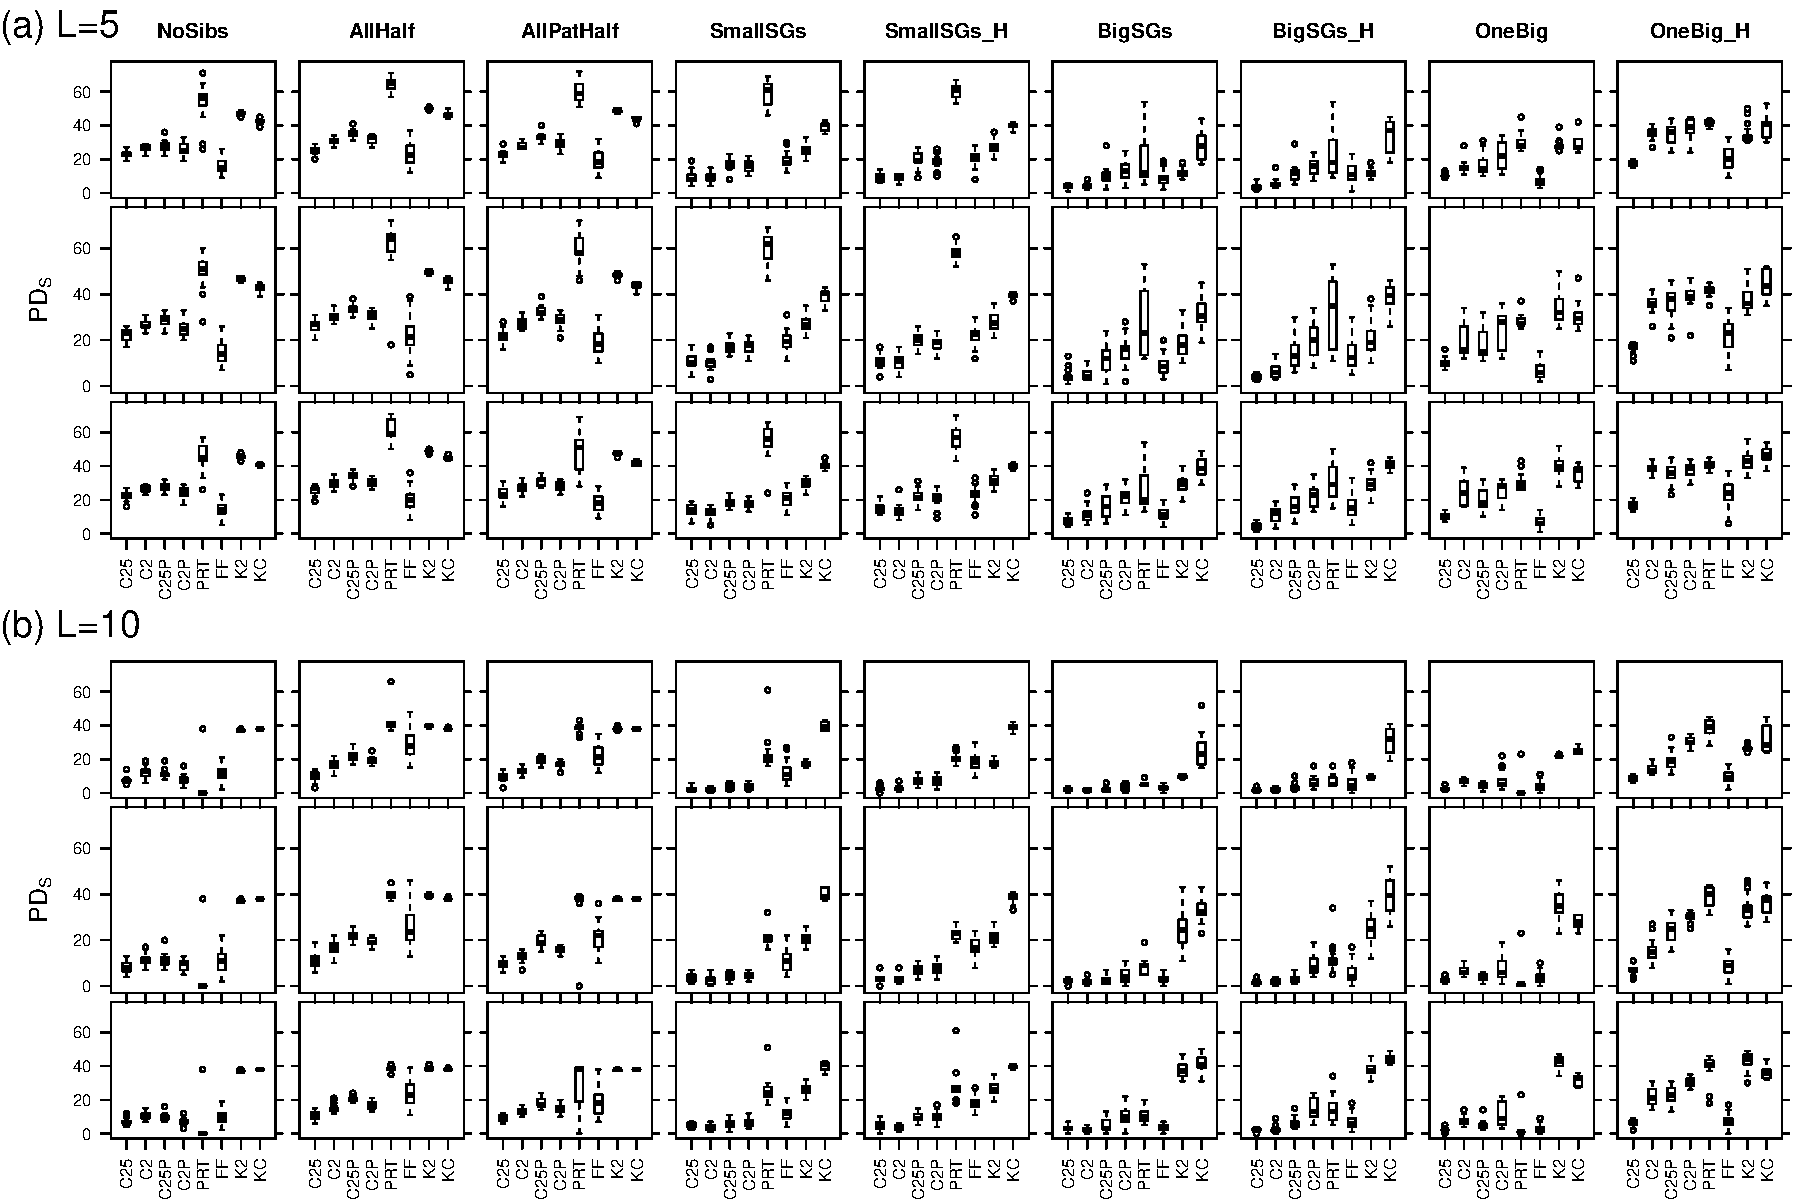
\includegraphics[width=\textwidth]{images/boxplots_for_paper10_num1.pdf}
\newcommand{\boxptwocaption}{Boxplot representation of values of $\PDS$ for $A=10$ alleles and $L=5$~({\em a}) and 
$L=10$~({\em b}). Format as in Figure~\protect\ref{fig:boxp1}.}
\caption[\boxptwocaption]{\sometimes{\boxptwocaption}}
\label{fig:boxp2}
\end{center}
\end{sidewaysfigure*}
%%
With such levels of data, which are perhaps closer to what might be employed in most sibship inference 
studies using microsatellites, we observe that \prt{} finds few spurious full sibling groups 
in the \nosibs{} case, outperforming both \colony{} and \colony{}-P in that scenario.
However, in the \allhalf{} and \allpathalf{} scenarios, which, like \nosibs{}, include no
full siblings, \colony{} and \colony{}-P outperform all the other programs.  As before, 
\familyfinder{} performs worse in the presence of half siblings than when half-siblings are absent (though 
relatively less poorly than with more informative data).  When half-siblings are not present, 
\familyfinder{} produces higher partition distances than it does with more informative data, just as 
one would expect.  The two \kinalyzer{} methods do quite poorly still.  
\prt{} continues to suffer higher error rates than \colony{}, \colony{}-P, or \familyfinder{} 
in the presence of small or moderately-sized full sibling groups.

With even less-informative data (such as $A=5$ and $L=5$, Figure~\ref{fig:boxp2}{\em a}) the performance of all methods is, predictably, 
degraded.  Interestingly, \prt{} no longer enjoys an advantage in the \nosibs{} case.  Rather, it erroneously infers very large sibling groups and performs worst of all the programs in the \nosibs{}, \allhalf{} and \allpathalf{} scenarios.  Supplement~3 contains a full set of boxplots for all the $n75$ simulation 
conditions.

\subsection*{$n75$ Scenarios---Detailed Comparisons}
Direct comparisons between pairs of inference methods on the same simulated data sets gives a useful 
sense of overall performance and helps to identify strengths and weaknesses of each method. A 
comprehensive display of such pairwise comparisons, broken down by simulation scenario and genotyping 
error rate, is available in Supplement~2. Across almost all of the scenarios, \colony~{\sc 2.0.5.2} performed 
as well or better than the other methods, so it is a natural choice for comparison.
Here, we will present and interpret several scatterplots comparing the performance of each method to 
\colony~{\sc 2.0.5.2} on all of the $n75$ simulated data sets at once.  Such a presentation loses a considerable 
amount of the information expressed in the figures of Supplement~2, but still captures important 
features.  Where it is helpful, we will refer readers to relevant individual figures in the 
Supplements.

We begin by comparing the performance of  \kinalyzer{}'s 2-allele algorithm to \colony{} on the 10,125 
$n75$ data sets that were analyzed with both programs.  In the scatterplots of Figure~
\ref{fig:cvksmear} each point represents a single data set; its $x$-coordinate is the partition 
distance between the \colony{} solution and the truth and its $y$-coordinate is the distance between 
the \kinalyzer{} solution and the truth.

%\begin{equation}
%\mbox{FIGURE ped\_configs\_figure.pdf}\label{fig:cvksmear}
%\end{equation}

\begin{figure*}
\begin{center}
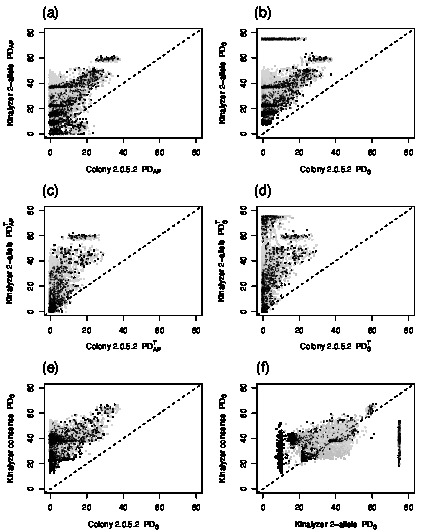
\includegraphics[width=.8\textwidth]{images/various_kina_smears.jpg}  %% Change extension from jpg to pdf for final version
\end{center}
\newcommand{\cvksmearcaption}{Scatterplots assessing performance of \kinalyzer{}.  {\em a}--{\em d} present comparisons of 
\colony{} versus \kinalyzer{}'s 2-allele algorithm for 10,125 simulated data sets, showing values of $
\W$, $\PDS$, $\WT$, and $\PDST$, respectively.  Thus, {\em b} and {\em d} penalize \kinalyzer{} for 
solutions that are not partitions, and {\em c} and {\em d} use the trimmed partition distances to 
lessen the impact of mistakes involving feasible sibling groups of size 2 or less. Each point 
represents the partition distances for a single data set with a small amount of uniformly-disributed 
jiggle (mean 0, min=-0.5, max=0.5) to separate points. Black points indicate data sets with no genotyping 
error; gray points denote data sets with genotyping errors. {\em e}) as above, but it compares 
\colony{} to \kinalyzer's consensus algorithm using $\PDS$.  {\em f}) comparison of \kinalyzer{}'s two 
methods: 2-allele versus consensus using $\PDS$.  Further discussion in text.}
\caption[\cvksmearcaption]{\sometimes{\cvksmearcaption}}
\label{fig:cvksmear}
\end{figure*}

Each of the four panels in Figure~\ref{fig:cvksmear}{\em a--d} summarizes the results for a different 
distance metric.  On the whole, it appears that \colony{} outperforms \kinalyzer{} regardless of which 
distance is used, but, as predicted, by failing to penalize for biologically impossible solutions, the 
$\W$ and $\WT$ formulations indicate that \kinalyzer{} performs better than it actually does.   
Nonetheless, even when assessing performance with $\W$ (Figure~\ref{fig:cvksmear}{\em a}), \colony{} 
performs as well or better than \kinalyzer{} on more than 94\% of the simulated data sets. 

There are three prominent features in Figure~2{\em a}.  The first is the distinct bands of black dots 
(indicating data sets with no genotyping error) at certain heights along the $y$-axis.  These 
correspond to unrelated individuals that \kinalyzer{} infers to be in sibships of size two.  For 
example, the prominent line at about $y=37$ is composed mostly of the three scenarios in which there 
are no full siblings. Since any two individuals will form a feasible sibling group, \kinalyzer{} has no 
basis for inferring that unrelated pairs are not full siblings, so large groups of unrelated 
individuals typically appear paired together (presumably at random) in \kinalyzer{}'s solutions.  Thus, 
if the truth is $n=75$ unrelated individuals and the \kinalyzer{} solution is 37 pairs of individuals 
and a singleton, then the \kinalyzer{} solution and the truth can be made identical by removing one 
individual from every pair; hence the line at $y=37$ in the plot. The second feature we notice is that, 
in general, simulating data sets with genotyping error (depicted with gray points) increases the error 
suffered by \kinalyzer{}.  Finally, the band of black and gray points at $y=0$ extending up to values 
of $x$ around 20 tells us that there are some data sets in which $\W$ is quite high for 
\colony{}, but is zero for \kinalyzer{}.  

Figure~\ref{fig:cvksmear}{\em b} plots values of $\PDS$, a metric which levies a penalty of 1 upon a 
solution for every individual that is inferred to be in more than one full sibship.  Most 
conspicuously, the band at $y=0$ present in Figure~\ref{fig:cvksmear}{\em a} is lacking in this panel.  
It has been replaced with a line at $y=75$.  Each point along this line indicates a solution returned 
by \kinalyzer{} in which {\em every} individual occurred in at least two sets in the set cover 
solution---in other words, {\em every} individual belonged to at least two distinct full sibling 
groups, defying biology.  We can conclude that the band at $y=0$ in Figure~2{\em a} does not indicate 
data sets where \kinalyzer{} enjoys an advantage, but rather it indicates data sets in which the
set-cover form of \kinalyzer{}'s solution attains its most pathological expression: every individual is 
included in at least two different full sibling groups.  Based on $\PDS$, \kinalyzer{} obtains a better 
result than \colony{} in none of the simulated data sets.

The occurrence of the horizontal line patterns in Figure~\ref{fig:cvksmear}{\em a} and {\em b} 
indicates that a large fraction of the errors made by \kinalyzer{} involve inferred sibships composed 
of unrelated individuals.  Some of these errors likely involve inferred sibships of size two, since 
\kinalyzer{} has no mechanism for distinguishing between unrelated individuals and sibships of size 
two.   However, Figure~\ref{fig:cvksmear}{\em c,d} reveals that, even using the trimmed partition 
distances, \kinalyzer{} is still outperformed by \colony{}.   In fact, based on $\PDST$, \kinalyzer{} 
did better than \colony{} in fewer than 0.3\% of the simulated data sets. 

We ran \kinalyzer{}'s consensus algorithm on 6,750 data sets and investigated the results.  In every 
case, the consensus algorithm returned a solution in the form of a true partition, rather than as a set 
cover; however, there was no clear advantage to using the consensus algorithm. \kinalyzer{}'s consensus 
option did not outperform \colony{} in any simulated data sets (Figure~
\ref{fig:cvksmear}{\em e}).  The consensus option does not appear to consistently  improve upon the 
results of the 2-allele algorithm in the presence of genotying error, and, in fact, often seems to 
produce poorer solutions than the 2-allele algorithm on data both with and without genotyping errors 
(Figures~\ref{fig:cvksmear}{\em f} and \ref{fig:Kinalyzer_v_KinaConsense_on_nosibs} through 
\ref{fig:Kinalyzer_v_KinaConsense_on_onelargewh}). 

\prt{}'s performance on individual data sets is compared to \colony~{\sc 2.0.5.2}'s in Figure~\ref{fig:cvffsmear}
{\em a,b}. 
%%%%
%\begin{equation}
%\mbox{FIGURE ped\_configs\_figure.pdf}\label{fig:cvffsmear}
%\end{equation}
\begin{figure*}
\begin{center}
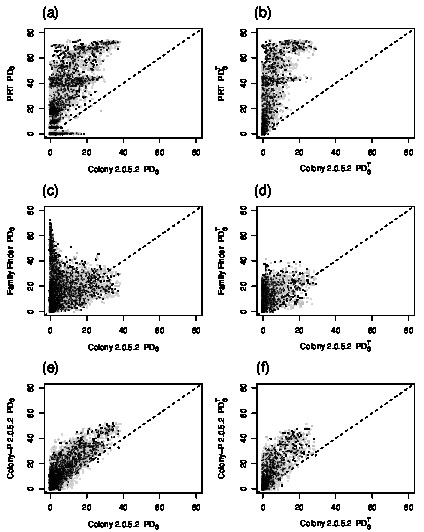
\includegraphics[width=.8\textwidth]{images/prt_ff_and_col_pair_smears.jpg}  %% Change extension from jpg to pdf for final version
\end{center}
\newcommand{\cvffsmearcaption}{Scatterplots comparing performance of \prt{} to \colony{} ({\em a,b}\/), \familyfinder{} 
to \colony{} ({\em c,d}\/), and \colony-P to \colony{} ({\em e,f}\/).  Figures are as in 
Figure~\protect\ref{fig:cvksmear}}
\caption[\cvffsmearcaption]{\sometimes{\cvffsmearcaption}}
\label{fig:cvffsmear}
\end{figure*}
%%%%
\colony{} achieves the same or a lower $\PDS$ than \prt{} on most (85.8\%) of the $n75$ data sets.  
Figures~\ref{fig:Colony2.0.5.2_v_PRT_on_nosibs} through \ref{fig:Colony2.0.5.2_v_PRT_on_onelargewh} show that 
the only cases where \prt{} consistently outperforms \colony{} are those with many unrelated individuals
 (\nosibs, \allhalf, \allpathalf, \onelargenoh, and \onelargewh). Inspection of the 
trimmed partition distances in these cases reveals that, when \prt{} outperforms \colony{}, it is because
\prt{} correctly infers no siblings in the data set while \colony infers a few to many incorrect sibling groups
of size 2.  
%THe   With only 5 alleles, regardless of 
%the number of loci, neither \colony{} nor \prt{} performed well on the \nosibs{} configuration, but 
%\colony{} tended to perform better.  With 10 alleles and 10 loci, however, \prt{} was more successful 
%than \colony{} at not inferring erroneous sibships in the \nosibs{} case (Figure~\ref{fig:boxp2}{\em 
%b}), and accordingly performed better than \colony{} in that situation.   
This is a consequence of 
\colony{}'s tendency to erroneously infer small sibling groups (pairs or trios) where there aren't any.  
This is confirmed by Figure~\ref{fig:cvffsmear}{\em b} which shows the band of dots at $y=0$ in Figure~
\ref{fig:cvffsmear}{\em a} is essentially eliminated when using $\PDST$, which does not penalize 
solutions for erroneously-inferred sibships of size 2. TALK ABOUT HOW THIS SEEMS TO APPLY TO A PARTICULAR BAND OF
DATA PARAMETERS. THEN UPDATE THE FOLLOWING PERCENTAGE. \colony{} achieves the same or a lower $\PDST$ 
as \prt{} on 96.6\% of the data sets.   

With more loci and with more alleles \colony{} generally performed as well as \prt{} in the \nosibs{} 
scenario, but consistently performed better than \prt{} regardless of the amount of data in cases where 
several small or medium-sized sibships occurred.  In these cases, since $\PDST$ was consistently less 
than $\PDS$ for \prt{} (Figures \ref{fig:Colony_v_PRT_on_sfsnoh} through 
\ref{fig:Colony_v_PRT_on_slfsgwh}), it is clear that many of the errors made by \prt{} involved the 
inference of incorrect sibships of size two. 

Additionally, Figures~\ref{xplot-a5l5} through \ref{xplot-a10l5} show that with relatively 
uninformative data, \prt{} has a tendency to infer very large, incorrect sibships (some including all 
the members of the sample) to a degree not seen in any of the other programs. This tendency may be due 
to the difficulty of correctly calibrating \prt{}'s new {\em post-hoc} method for handling genotyping 
errors.  Features in Figure~\ref{fig:Colony_v_PRT_on_slfsgnoh} suggest that the method for handling 
genotyping errors might be difficult to calibrate---it is clear that with no genotyping error, \prt{} 
performs better on data sets with many markers, but with genotyping error, there is a clear shift 
apparent, and the data sets with more loci actually  have relatively higher $\PDS$ than their 
counterparts with fewer loci. 




\familyfinder{} compares more favorably to \colony{} (Figure~\ref{fig:cvffsmear}{\em c,d}) than does 
\kinalyzer{}, performing in the aggregate about as well as \prt{} against \colony{}. 
\colony{}'s $\PDS$ is equal or less than \familyfinder{}'s in 79\% of the simulated data sets.
A prominent feature in Figure~\ref{fig:cvffsmear}{\em c} is the band of black dots reaching almost to 
$y=75$ near $x=0$.  These are data sets in which \colony{}'s solutions are near perfect, but 
\familyfinder{} makes many errors.  Most of those points are from the \allhalf{} and \allpathalf{} 
scenarios and the higher $y$-values correspond to data sets with more loci (Figures~
\ref{fig:Colony_v_FamilyFinder_on_allhalf}, \ref{fig:Colony_v_FamilyFinder_on_allpathalf}).  
Effectively, with more data, \familyfinder{} is more likely to mistake large half-sibling groups as 
large full sibling groups.  The fact that the band of dots does not appear using the trimmed partition 
distance (Figure~\ref{fig:cvffsmear}{\em d}) indicates that many of the erroneous full sibling groups 
found by \familyfinder{} in the \allhalf{} and \allpathalf{} scenarios consist of only two individuals.   
Also apparent in Figure~\ref{fig:cvffsmear}{\em c,d} is a cloud of points below the $y=x$ line, where 
neither \familyfinder{} nor \colony{} find accurate solutions, but \familyfinder{} tends to do better 
than \colony{}.  Figures~\ref{fig:Colony_v_FamilyFinder_on_nosibs} through 
\ref{fig:Colony_v_FamilyFinder_on_onelargewh} reveal that these points are predominantly from data sets 
with few markers and few alleles ($\leq 10$ of each) from the scenarios \allhalf{}, \allpathalf{}, 
\nosibs{}, \onelargenoh{}, and \onelargewh{}\@.  Notably, all of these scenarios include large numbers 
($\geq$ 45) of individuals who are unrelated or are half siblings, and, in fact, most of the partition 
distance in these cases is due to the fact, identified above, that given a small number of genetic 
markers with low diversity, \colony{} tends to infer small full sibling groups composed of unrelated or 
half-sib individuals (see, for example, Figure~\ref{xplot-a5l5}).  

Figures~\ref{fig:Colony_v_FamilyFinder_on_onelargenoh} and 
\ref{fig:Colony_v_FamilyFinder_on_onelargewh} further show that \familyfinder{} compares favorably with 
\colony{} (if not carrying a small advantage with few loci and alleles) when seeking a single large sibling group amongst 
otherwise unrelated individuals (\onelargenoh) or amongst half siblings (\onelargewh).  This pattern is 
even more apparent in the boxplots of Figure~\ref{fig:boxp1}.  However, \colony{} far outperforms 
\familyfinder{} when the sample is composed of many small full sibling groups (\sfsnoh), especially in 
the presence of half siblings (\sfswh), and \colony{} appears to have a moderate advantage when the 
sample is a mixture of large and small sibling groups (\slfsgnoh) which becomes a much larger advantage 
in the presence of half siblings (\slfsgwh).

    
Of all the competing methods, \colony-P's performance is most closely correlated with that of \colony{} 
(Figure~\ref{fig:cvffsmear}{\em e,f}).  Comparing the number of points below the $y=x$ line using $\PDS
$ (Figure~\ref{fig:cvffsmear}{\em e}) to that using $\PDST$ (Figure~\ref{fig:cvffsmear}{\em f}), it is 
clear that when \colony{}-P achieves a lower partition distance than \colony{} it is in those cases 
where \colony{} is erroneously inferring sibships of size~2.  Inspection of Figures~
\ref{fig:Colony_v_ColonyP_on_nosibs} through \ref{fig:Colony_v_ColonyP_on_onelargewh} make it clear 
that almost all of the data sets in which \colony{}-P outperforms \colony{} are in the \nosibs{} or 
\onelargenoh{} categories---situations in which there are many unrelated individuals.  Once again, 
these are situations where \colony{} erroneously infers small sibships from unrelated individuals.  In 
all other situations, as expected, \colony{} enjoys an advantage, especially with lower numbers of 
markers and alleles and also in the presence of half siblings (see \ref{fig:Colony_v_ColonyP_on_nosibs} 
through \ref{fig:Colony_v_ColonyP_on_onelargewh}). Overall, \colony{} performed as well or better than 
\colony{}-P in 88\% of the data sets on the basis of $\PDS$ and in 94\% of the data sets on the basis 
of $\PDST$.

\subsection*{$n75$ Scenarios---Running Times}
There was a wide disparity between the running times of the different programs (Table~
\ref{tab:n75times}). 
%%
\begin{table*}
\caption{Running times in minutes averaged over all $n75$ data sets analyzed for $A=15$ and 
$L$ as indicated. Slant font gives the 10\% and 90\% quantiles.\label{tab:n75times}}
\begin{center}
\begin{tabular}{lccccc}
\hline
  & \multicolumn{5}{c}{\underline{Number of Loci ($L$)}} \\
        & 5  &  10  &  15  &  20  &  25 \\ \hline
\colony{}$^a$  &  5.45  &  12.15  &  20.02  &  28.18  &  35.93 \\
           &  {\sl 4.06--6.68}  &  {\sl 7.68--18.33}  &  {\sl 12.01--33.63}  &  {\sl 16.21--49.16}  &  {\sl 20.79--63.18} \\
\colony{}-P$^a$  &  1.54  &  1.52  &  1.48  &  1.46  &  1.43 \\
           &  {\sl 1.17--2.04}  &  {\sl 1.10--2.03}  &  {\sl 1.07--1.98}  &  {\sl 1.07--1.95}  &  {\sl 1.05--1.96} \\
\prt{}$^b$  &  4.00  &  1.44  &  0.98  &  1.51  &  0.94 \\
        &  {\sl 0.37--9.65}  &  {\sl 0.25--1.73}  &  {\sl 0.24--1.46}  &  {\sl 0.26--1.52}  &  {\sl 0.28--1.53} \\
\familyfinder{}$^a$  &  $<1$ sec  &  $<1$ sec  &  $<1$ sec  &  $<1$ sec  &  $<1$ sec \\
\kinalyzer{}$^c$  &  0.52  &  1.32  &  16.61  &  49.86  &  134.99 \\
              &  {\sl 0.45--0.58}  &  {\sl 0.65--2.45}  &  {\sl 0.65--43.93}  &  {\sl 17.84--78.72}  &  {\sl 66.97--166.62} \\
\hline
\end{tabular}
\end{center}
{\footnotesize $^a$Times listed are total clock times for each job.  Since each job was run on
a dedicated processor, this will be close to {\em user} + {\em system} time.}\\
{\footnotesize $^b${\em user} times}\\
{\footnotesize $^c$Running times for \kinalyzer{} are approximate. \kinalyzer{} does not report
the amount of computing resources used. Times listed here are the differences between the time
that the job was submitted and the time that the result was emailed back to us. }
\end{table*}
%%
The fastest program was \familyfinder{} which never required more than one second to analyze any of the 
$n75$ data sets, regardless of the number of loci used.   \colony{}-P's run time was relatively 
unaffected by the number of loci, being, on average, 1.5 minutes when $A=15$.  This is to be expected, 
as the approximation made in \colony{}-P permits the program to proceed without the need to recalculate 
likelihoods at each locus whenever it proposes a new sibling configuration of the data.  \prt{}'s run 
times for data sets with 5 loci were higher than with 10 loci but running times with more loci were 
relatively constant and comparable to \colony-{}P's at about 1 to 1.5 minutes. By contrast, \colony{} 
showed a roughly linear increase in computing time with number of loci (35 minutes with 25 loci), and 
\kinalyzer{}'s run times appear to increase exponentially with the number of loci; for $L=25$  
\kinalyzer{} returned its result in 135 minutes, on average.  Detailed plots of run times for all the 
different data scenarios are found in Supplement~5.




\subsection*{\lottalarge{} Scenarios}
%

%\begin{equation}
%\mbox{FIGURE ped\_configs\_figure.pdf}\label{fig:llboxp}
%\end{equation}

\begin{sidewaysfigure*}
\begin{center}
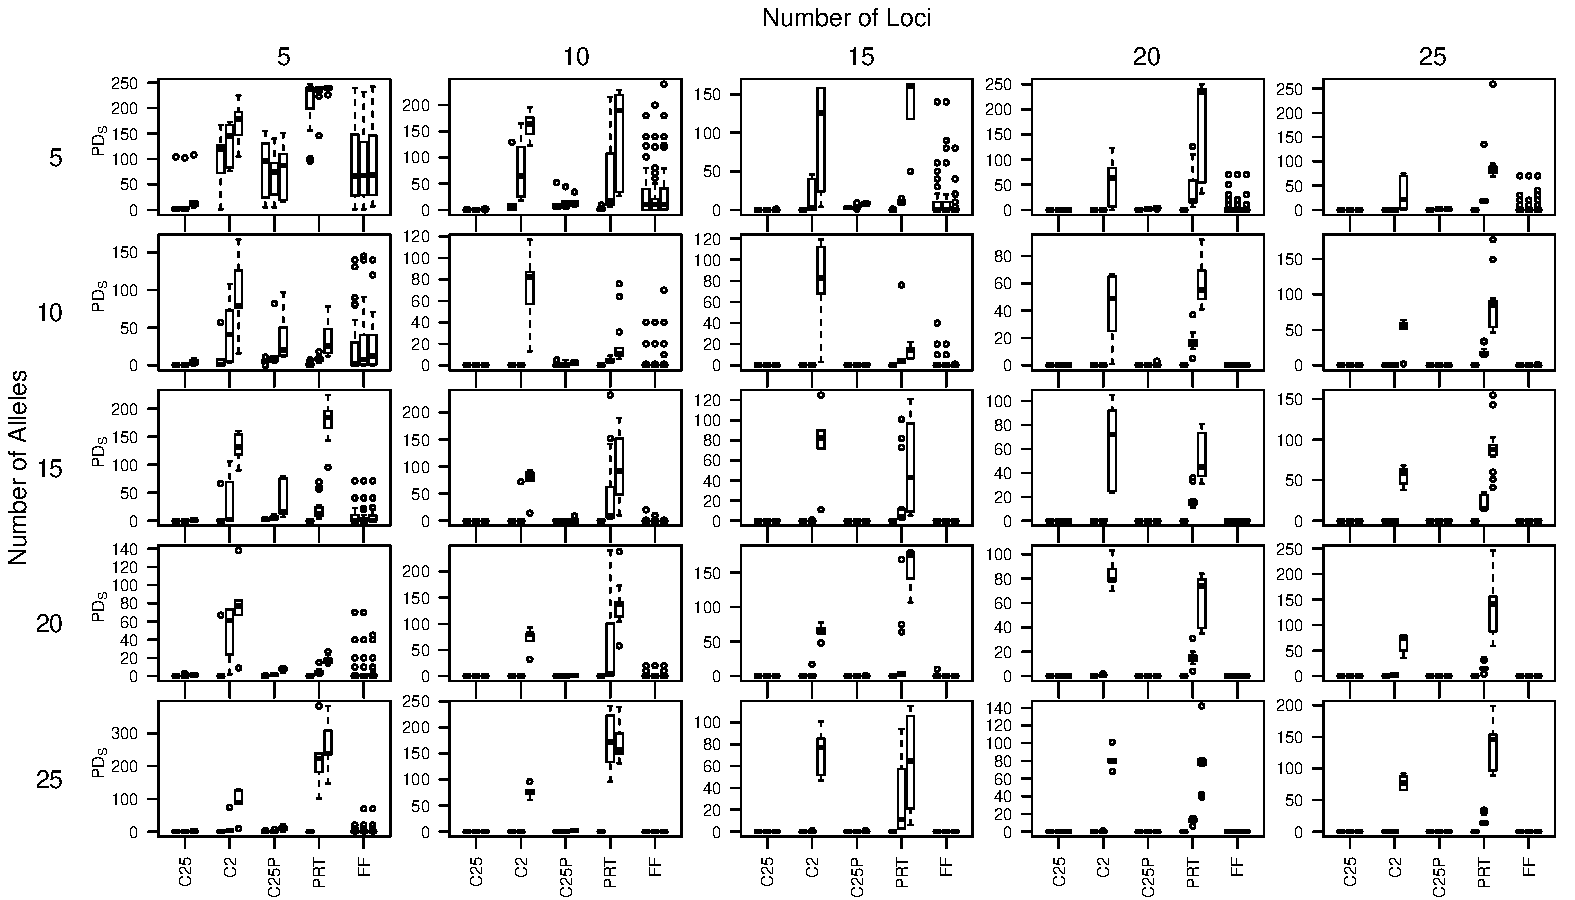
\includegraphics[width=\textwidth]{images/lotta_large_boxplots.pdf}  
\end{center}
\newcommand{\llboxpcaption}{Boxplot representation of values of $\PDS$ for on \lottalarge scenarios with $A$ and $L$ 
varying in rows and columns, respectively.  For each method (CO=\colony{}, CP=\colony-P, PRT=\prt, and 
FF=\familyfinder) three box plots are given.  The leftmost is for data with no genotyping error; the 
center with $d=0.02$,~$m=.01$, and the rightmost with $d=0.07$,~$m=.03$.  Note that for some values of 
$A$ and $L$, \prt{} failed to complete on any data sets, which is indicated by the absence of the 
boxplot in those cases. }
\caption[\llboxpcaption]{\sometimes{\llboxpcaption}}
\label{fig:llboxp}
\end{sidewaysfigure*}

%
The data from the \lottalarge{} scenario included 390 individuals in several very large full sibships 
with no half-siblings.  With no genotyping error, \colony{} made nearly no errors except for a small
handful with $A=5,\ L=10$ and $A=10,\ L=5$, and substantially more (as expected) with $A=L=5$.  The other 
programs (\colony-P{}, \prt{}, and \familyfinder{}) 
also made almost no errors (performing as well or nearly as well as \colony{}) so long as the data 
included at least
10 alleles and 10 loci. As the genotyping error
rate increases, there is more spread in program performance.  With moderate genotyping error 
($d=0.02,~m=0.01$) \colony{} is the best-performing method when both $L$ and $A$ are $\geq~10$, with 
\familyfinder{} performing nearly as well in these cases, and \prt{} suffering some evident
inaccuracy at higher locus numbers.  With high genotyping error rates ($d=0.07,\ m=0.03$), 
\familyfinder{} enjoys the highest level of accuracy across almost all conditions.  \colony{}, in these
cases, suffers from splitting of the large (150-member) full sibling group. As seen 
in Figure~\ref{fig:new-colony-boxp}, this
splitting is virtually eliminated in the most recent version, \colony{}-2.0.5.0
\citep{Wang2013}, such that even at very high levels of genotyping error \colony{} makes no errors at 
$A=10$ and thus outperforms
all the other methods.
% New version of colony 10-locus boxplot figure
\begin{figure*}
\begin{center}
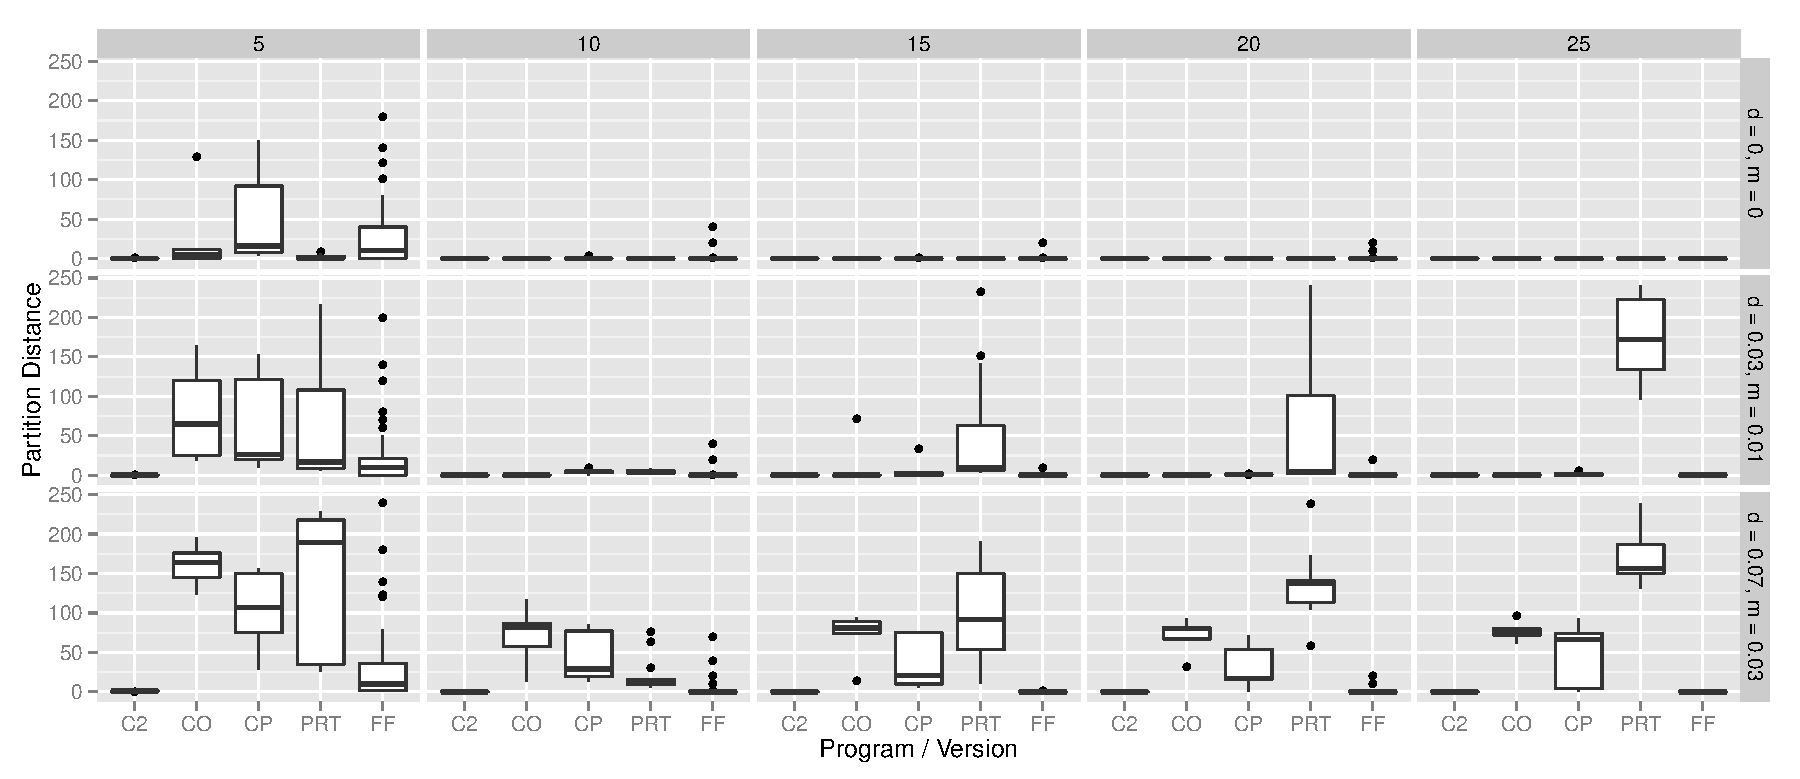
\includegraphics[width=\textwidth]{./images/new-colony-boxplots-10-loci.pdf}
\end{center}
\newcommand{\newcolonyboxcaption}{Boxplots of $\PDS$ for $A=10$ in the \lottalarge{} scenario including
results for \colony{}-2.0.5.0. 
Different rows are different genotyping error rates and the columns are different numbers of loci. Names 
of methods are C2=\colony{}-2.0.5.0, CO=\colony{}, CP=\colony-P, PRT=\prt, and 
FF=\familyfinder).  Note in particular that, even with high genotyping error rate, $\PDS$ is reduced 
to near 0 in C2, indicating that the method of \citet{Wang2013} successfully avoids splitting 
large sibling groups in these data sets.} 
\caption[\newcolonyboxcaption]{\sometimes{\newcolonyboxcaption}}
\label{fig:new-colony-boxp}
\end{figure*}


Running times on the \lottalarge{} data appear in \ref{fig:run-time-noki-lotta_large}.  \familyfinder{} 
never required more than 4.1 seconds to complete, and averaged 2.5 seconds across all data sets of the 
\lottalarge{} scenario.  By contrast, \colony{} typically required from 1 to 2 hours to complete each 
data set, and, with many loci, sometimes three to four times that. Excluding those cases when it failed 
to return a result, \prt{} typically required running times measured in minutes.

\section*{Discussion}
We have provided a comprehensive evaluation of six different full sibling inference
methods---\colony{}, \colony-P, \familyfinder{}, \kinalyzer{} (2-allele), \kinalyzer{} (consensus), 
and \prt{}---by applying the methods to thousands of simulated data sets covering a broad range of number of loci 
and alleles, relationship configurations, and genotyping error rates.  We evaluated each solution by 
comparing it to the true full sibling structure of the data on the basis of the partition distance.  
There was no single method that performed best across all of the simulation scenarios; however several 
strong patterns in the results imply a number of reliable recommendations.

The most consistent pattern in the results was the uniformly poor performance of \kinalyzer{}, both in 
its ``2-allele'' and its ``consensus'' forms.  It almost never performed better than any of the other 
methods across any of the simulation scenarios.  Furthermore, when presented with very informative data 
(many alleles and loci), it performed considerably worse than the best programs, and had very long run 
times.  We identified no situations for which we can recommend the use of \kinalyzer{}.

When full siblings existed in the sample, the program \colony{} performed best at identifying them.  
This result was consistent across scenarios (with or without half siblings) and across numbers of 
alleles and loci.  However, this sensitivity to full siblings comes at the cost of a lack of 
specificity.  The program \colony{} was occasionally outperformed in scenarios that included no full 
siblings.  We have previously discussed the need for statistical error control in 
sibship inference \citep{alm&and11}, pointing out that for any given number of loci and alleles, there 
exists a sufficiently large sample that some unrelated individuals will form feasible sibling groups 
(and will have high likelihood of being full siblings).  It might be hoped that \colony{}'s {\em ad 
hoc} confidence calculation (which approximates the posterior probability of inferred sibling 
configurations based on states visited during simulated annealing) would assign a low confidence to 
incorrect sibling groups; however our results suggest this is not the case. With $N=75$ unrelated 
individuals, \colony{} identifies many high-confidence (posterior probability $\geq 0.98$) full sibling 
pairs, and even trios, depending on the number of loci and alleles (Table~\ref{tab:hiconf}).
Applying the same number of loci and alleles to a larger sample of unrelated individuals, \colony{} is 
expected to infer even more erroneous sibling groups with high ``confidence."

The latest version of \colony{} not only reduces splitting of large sibling groups, but also applies
a correction to reduce the inference of spurious small sibling groups.  A limited set of runs 
with \colony{}-2.0.5.0 on data from the \nosibs{}, \allhalf{} and \allpathalf{} scenarios with $A=10$ 
and $L\in\{5,10\}$ confirms that the correction consistently reduces the occurrence of small spurious 
sibling groups, but does not eliminate it altogether (Figures~\ref{fig:OldColony_v_NewColony_on_nosibs} 
and~\ref{fig:OldColony_v_NewColony_on_allhalf}). Another option would be to use \colony{}'s Ewens' prior to 
penalize small sibling groups if large groups were expected.  However this could be difficult
in cases where little information is available {\em a priori} on expected sibship sizes.


Clearly, \colony{}'s results should be used with caution when it has inferred a small number of 
small sibling groups.  In fact, we recommend that \colony{}'s output not be used as the sole method 
to infer pairs or trios of full siblings from amongst a much larger sample. For such cases, there are 
more powerful methods that also include statistical error control (see, for example, 
\citealt{almudevar01b}).  Additionally, when confronted with a \colony{} result suggesting that only a 
few small sibships exist, it is worthwhile comparing that result to the result \colony{} obtains on a 
data set that matches the original in terms of genetic diversity, number of loci, and missing data, but 
in which it is known that all individuals are completely unrelated.  This can be achieved by fixing 
missing data in place in the original data set and then permuting the alleles within each locus amongst 
all the members of the sample, and analyzing the result with \colony{}. If \colony{} continues to find 
small sibling groups in the permuted data, then this should reduce one's confidence
regarding \colony{}'s results for 
the original data set.  Alternatively, \colony{} 
itself now offers a simulation module that can assist in interpreting 
\colony{}'s results (see \citealt{Wang2013simulation}).

%%
\begin{table*}[t!]
\caption{High-confidence errors in \colony{}. Across 15 simulated data sets of size $n=75$,
the average number of full sibships of size $S$ inferred with posterior probability $\geq 0.98$ by
\colony{}. Simulations were done without genotyping error using the \nosibs{} and the
\allhalf{} configurations as indicated; both configurations have no true full sibling groups in
them.  Column $L$ holds number of loci.  \label{tab:hiconf}  } 
\begin{center}
\begin{tabular}{crrrrrrrrrrrr}
\hline
                &      & \multicolumn{5}{c}{\underline{Number of Alleles}}      &    & \multicolumn{5}{c}{\underline{Number of Alleles}}       \\
$S$  &  $L$  &  5  &  10  &  15  &  20  &  25  &    &  5  &  10  &  15  &  20  &  25\\
2  &  5  &   9.67  &   9.20  &   7.67  &   6.00  &   4.67  &    &   8.67  &  10.20  &  10.27  &   8.93  &   7.00\\
  &  10  &   6.87  &   3.80  &   1.40  &   0.93  &   0.33  &    &   7.60  &   4.33  &   1.20  &   0.40  &   0.20\\
  &  15  &   2.87  &   0.47  &   0.20  &   0.07  &   0.00  &    &   3.67  &   1.13  &   0.00  &   0.07  &   0.00\\
  &  20  &   1.07  &   0.07  &   0.00  &   0.00  &   0.00  &    &   1.20  &   0.07  &   0.00  &   0.00  &   0.00\\
  &  25  &   0.27  &   0.00  &   0.00  &   0.00  &   0.00  &    &   0.20  &   0.00  &   0.00  &   0.00  &   0.00\\
  &    &    &    &    &    &    &    &    &    &    &    &  \\
3  &  5  &   2.13  &   1.80  &   0.60  &   0.27  &   0.07  &    &   2.73  &   2.00  &   1.07  &   0.60  &   0.47\\
  &  10  &   0.47  &   0.07  &   0.00  &   0.00  &   0.00  &    &   0.87  &   0.07  &   0.00  &   0.00  &   0.00\\
  &  15  &   0.00  &   0.00  &   0.00  &   0.00  &   0.00  &    &   0.07  &   0.00  &   0.00  &   0.00  &   0.00\\
  &  20  &   0.00  &   0.00  &   0.00  &   0.00  &   0.00  &    &   0.00  &   0.00  &   0.00  &   0.00  &   0.00\\
  &  25  &   0.00  &   0.00  &   0.00  &   0.00  &   0.00  &    &   0.00  &   0.00  &   0.00  &   0.00  &   0.00\\
  &    &    &    &    &    &    &    &    &    &    &    &  \\
$\geq 4$  &  5  &   1.00  &   0.20  &   0.00  &   0.00  &   0.00  &    &   0.93  &   0.27  &   0.13  &   0.00  &   0.00\\
  &  10  &   0.00  &   0.00  &   0.00  &   0.00  &   0.00  &    &   0.00  &   0.00  &   0.00  &   0.00  &   0.00\\
  &  15  &   0.07  &   0.00  &   0.00  &   0.00  &   0.00  &    &   0.00  &   0.00  &   0.00  &   0.00  &   0.00\\
  &  20  &   0.00  &   0.00  &   0.00  &   0.00  &   0.00  &    &   0.00  &   0.00  &   0.00  &   0.00  &   0.00\\
  &  25  &   0.00  &   0.00  &   0.00  &   0.00  &   0.00  &    &   0.00  &   0.00  &   0.00  &   0.00  &   0.00\\

\cline{3-7} \cline{9-13}
                &      & \multicolumn{5}{c}{\nosibs}                &    & \multicolumn{5}{c}{\allhalf}       \\ 
\hline
\end{tabular}
\end{center}
\end{table*}
%% 
For some values of $L$ and $A$, \prt{} was much better than \colony{} at inferring no sibships when 
there were none; however this behavior was not consistent across all $L$ and $A$.  For some values of 
$L$ and $A$, \prt{} inferred very large sibling groups where none existed. In fact, it was very 
difficult to predict the behavior of \prt{}.  For several scenarios \prt{} did best with an 
intermediate amount of data: too little and its inferences were unreliable, too much and it might not 
complete its calculations.  Unfortunately, it is not always straightforward to predict the scenarios in 
which \prt{} will perform well.  Some of the inconsistency of \prt{}'s performance may be due to issues 
of tuning the value of $K$---the number of allowed genotyping errors per individual---in \prt{}'s 
recently developed method for handling genotyping errors (Appendix~1).

\colony{} also requires that the user set a genotyping error parameter.  We performed a series of 
\colony{} runs to explore the effect of misspecification of this error rate.  We found that, although 
setting the assumed error rate to zero produced poor results when genotyping error was present, there 
was relatively little difference in the results between different non-zero values of the error rate 
setting (\ref{fig:ColMed_v_ColNone_on_nosibs} through \ref{fig:ColMed_v_ColHigh_on_onelargewh}).

Previous work has noted that \colony{} may have a tendency to erroneously split large full sibling groups
\citep{alm&and11}.  In our $n75$ simulations, we did not observe excessive amounts of such
splitting. An updated version of \colony{} now employs a correction
to avoid splitting of large true full sibships \citep{Wang2013}.  Since we did not observe 
much splitting with the old version of \colony{}, use of the new version would unlikely change
our results in the $n75$ scenarios greatly.  However, a limited number of runs on several
\lottalarge{} data sets confirmed
that this updated version of \colony{} does not split large sibling groups in cases where the
old version does.


For reasons of computational efficiency, we did not use the setting in \colony{} introduced in
\citet{wang09} allowing both sexes to by polygamous.  This setting would likely have
improved \colony{}'s performance in cases when both sexes are polygamous, like \allhalf{}. Additionally,
in this paper we have focused on the inference of full sibling groups. Inference of half-siblings 
is a harder problem.  It is worth noting that \colony{}'s model, unlike any of the other softwares
assessed here, jointly infers full and half-sibling groups.  One of the great advantages of this 
is that half-sibling groups can be identified more accurately if there are large full sibling
groups nested within half-sibships.  Thus, half-siblings may be found more confidently by exploiting
this joint inference.


\colony-P \citep{Wang2012pairwise} is considerably faster than \colony{} for data sets with
many individuals, and performs as well, relative to \colony{}, as any of the other methods.
However, \colony{} is almost uniformly more accurate than 
\colony-P, especially in the presence of half-siblings. Therefore, with small numbers of 
individuals (100s) \colony{} would be preferred over \colony-P.  When sample sizes enter
the 1,000's, though, \colony{}'s run times can become prohibitive, and \colony-P is a
useful alternative in those cases.  

The ability to gather large data sets is 
increasing rapidly, so approximate methods that are computationally efficient yet
perform well when given a large number of polymorphic markers 
will likely become increasingly relevant.
\familyfinder{} was orders of magnitude faster than any other program, and, with large numbers of 
markers and alleles it performed as well as \colony{} when there were no half-siblings present.  It 
will be interesting to investigate (as suggested by \familyfinder{}'s authors) modifications to the
program to
explicitly take account of the occurrence of half-siblings.  With such modifications,
\familyfinder{}'s accuracy could approach that of \colony{}'s,
at least in cases with many, very informative markers.


Overall, \colony{} consistently performed well when
there were actually siblings in the data set.  
Given data of sufficient quality
\prt{} can be generally recommended for cases where there is a single large
sibling group. For example, with $A\geq 10$ and $L\geq 15$ 
in the \onelargenoh{} scenario, \prt{} appears to be consistently 
accurate, although the accuracy of \colony{} 
and \familyfinder{} are comparable; however the introduction of 
half-siblings in the \onelargewh{} case presents more difficulty for
\prt{} than for \colony{}.  
Interestingly, given its emphasis on large 
sibling groups, \prt{} consistently performs as well, or better, than all other algorithms for the 
\nosibs{}, \allhalf{}, and \allpathalf{} scenarios when $A\geq10$ and $L\geq15$. 
For scenarios with many large full sibling group, such as \slfsgnoh{} and \slfsgwh{},
\colony{} offers the best accuracy, consistently, though \colony{}-P, \familyfinder{}, and 
\prt{} remain viable alternatives.  
For these latter two scenarios, memory requirements sometimes hampered the 
performance of \prt{}. For especially large problems careful tuning of memory parameters will be 
required. 
When samples include many small full sibling groups, such as in the \sfsnoh{} and  \sfswh{} scenarios, \colony{} and \colony-P were consistently most accurate.   
We found no scenarios for which we could recommend the use of \kinalyzer{}.


We did not assess the performance of these methods when using data on biallelic
markers, like SNPs.  The explosion of next generation sequencing data 
in molecular ecology suggests that very soon it will be possible to 
generate large data sets with every individual typed at 100's to 1,000s
of SNPs.  Methods like \prt{} and \kinalyzer{} that rely on Mendelian 
incompatibility to assist in the inference of sibling groups will not
be effective for SNP data. Furthermore, none of the methods we reviewed 
has a mechanism for accounting for physical linkage of the markers.
However, given that the amounts of data available
could be very large, approximate approaches based on pairwise likelihoods,
like \familyfinder{}, may prove useful for efficiently handling 
large numbers of SNP markers.




\section*{Acknowledgments}
We are grateful for Jinliang Wang's careful reading of an earlier draft of our manuscript and his very helpful
comments and corrections.  We also acknowledge helpful correspondence with Tanya Berger-Wolf.
